\subsection{Baza danych }
\subsubsection{Data}
25.03.2019
\subsubsection{Osoby odpowiedzialne}
Jan Niewiarowski, Mateusz Skowronek

\subsubsection{Specyfikacja}
Lokalna baza danych została zaimplementowana na silniku MongoDB. Silnik MongoDB jest przykładem bazy niewykorzystującej języka SQL oraz nierelacyjnej. Charakteryzuje się dużą skalowalnością, wydajnością oraz brakiem ściśle zdefiniowanej struktury obsługiwanych baz danych. MongoDB składuje dane w postaci plików JSON, które nazywa dokumentami i umieszcza je w tzw. kolekcjach. Silnik nie wymaga tworzenia schematu bazy danych lecz wstawia dokument JSON do kolekcji, która jeżeli nie istnieje zostaje automatycznie utworzona. 
\newline
W porównaniu z relacyjną bazą danych, np. MySQL, MongoDB jest prostsza i wydajniejszy. Przy użyciu tego silnika można skalować bazę na wiele serwerów.
Dodatkowo bazę można podłączyć i skonfigurować z wieloma różnymi językami programowania, np. Java lub JavaScript.
\newpage

\begin{figure}[h!]
  \centering
    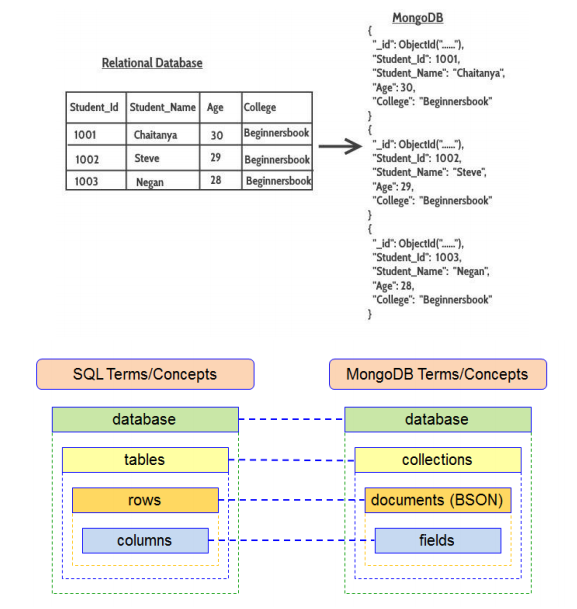
\includegraphics[width=0.95\textwidth]{img/mongo.png}
  \caption{Porównanie relacyjnej bazdy danych z MongoDB} 
  \label{fig:org}                                       
\end{figure}

\newpage

\subsubsection{Kolekcje w bazie danych}
W bazie danych przechowywane będą elementy takie jak: \\
- pomiar czujników (puls i saturacja), \\
- dane poszkodowanego (numer identyfikacyjny, priorytet według zasad triage, lokalizacja, informacje dodatkowe), \\
- informacje konieczne do wypełnienia karty działań kierującego akcją medycznych czynności ratunkowych (KAM), \\
- informacje potrzebne do wypełnienia karty działań dyspozytora medycznego kierującego (DM-K), \\


\subsubsection{Przykładowe kolekcje znajdujące się w bazie}


Dane czujnika:
\begin{verbatim}
sensorInfo = {
    "priority" : enum,
    "lifeFunctionSeries": [
        {
            "timestamp" : unxiTimestamp,
            "pulse":  number,
            "saturation": number,
        }
    ]
}
\end{verbatim}
Dane poszkodowanego:
\begin{verbatim}
victimInfo = {
    "id" : number,
    "priorityHistory": [
        {
            "priorty" : enum,
            "timestamp": unixTimestamp
        }
    ],
    "sensorInfo": sensorInfo,
    "lastKnownCoordinates": GPS,
    "rescueTeamId": string,
    "assignedHospital": string,
    "injuries": string,
    "additionalInfo": string    
}
\end{verbatim}
\newpage
\subsubsection{Karta działań dyspozytora medycznego kierującego (DM-K)}

\begin{figure}[h!]
  \centering
    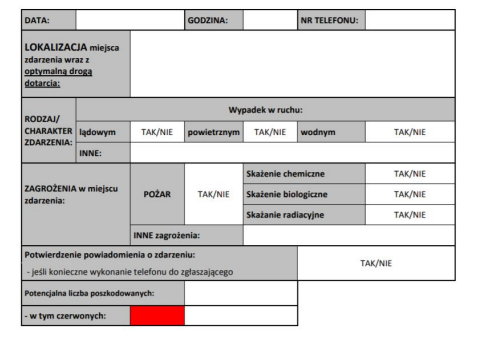
\includegraphics[width=0.95\textwidth]{img/powiadomienia.png}
  \caption{Powiadomienie} 
  \label{fig:org}                                       
\end{figure}

\begin{figure}[h!]
  \centering
    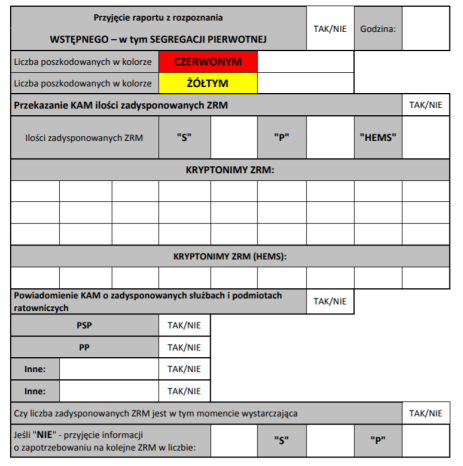
\includegraphics[width=0.95\textwidth]{img/Kamtodmk.png}
  \caption{Wymiana informacji pomiędzy KAM a DM-K} 
  \label{fig:org}                                       
\end{figure}

\begin{figure}[h!]
  \centering
    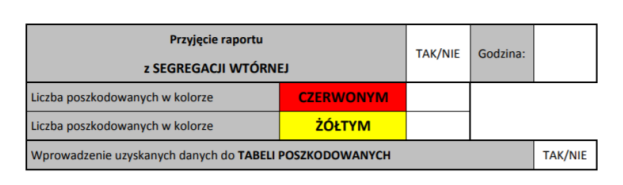
\includegraphics[width=0.95\textwidth]{img/Kamtodmk2.png}
  \caption{Wymiana informacji pomiędzy KAM a DM-K} 
  \label{fig:org}                                       
\end{figure}

\begin{figure}[h!]
  \centering
    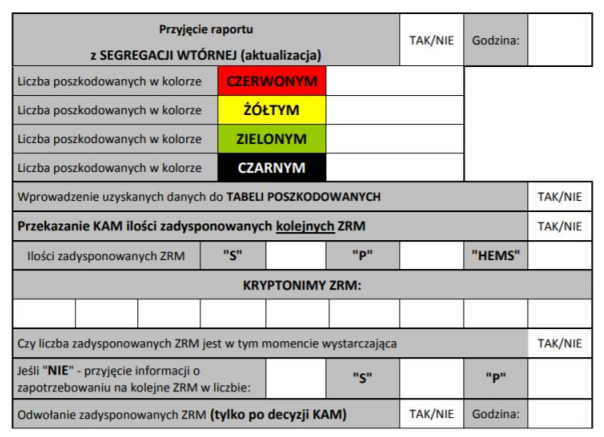
\includegraphics[width=0.95\textwidth]{img/Kamtodmk3.png}
  \caption{Wymiana informacji pomiędzy KAM a DM-K} 
  \label{fig:org}                                       
\end{figure}

